\documentclass[a4paper,14pt]{extarticle}

\usepackage[utf8x]{inputenc}
\usepackage[T1]{fontenc}
\usepackage[russian]{babel}
\usepackage{hyperref}
\usepackage{indentfirst}
\usepackage{here}
\usepackage{array}
\usepackage{graphicx}
\usepackage{caption}
\usepackage{subcaption}
\usepackage{chngcntr}
\usepackage{amsmath}
\usepackage{amssymb}
\usepackage[left=2cm,right=2cm,top=2cm,bottom=2cm,bindingoffset=0cm]{geometry}
\usepackage{multicol}
\usepackage{multirow}
\usepackage{titlesec}
\usepackage{listings}
\usepackage{color}
\usepackage{enumitem}
\usepackage{cmap}
\usepackage{underscore}

\definecolor{green}{rgb}{0,0.6,0}
\definecolor{gray}{rgb}{0.5,0.5,0.5}
\definecolor{purple}{rgb}{0.58,0,0.82}

\lstdefinelanguage{none}{}

\lstset{
	language={C++},
	inputpath={../generator/src/main/java/com/vaddya/hotelbooking},
	backgroundcolor=\color{white},
	commentstyle=\color{green},
	keywordstyle=\color{blue},
	numberstyle=\scriptsize\color{gray},
	stringstyle=\color{purple},
	basicstyle=\ttfamily\small,
	breakatwhitespace=false,
	breaklines=true,
	captionpos=b,
	keepspaces=true,
	numbers=left,
	numbersep=5pt,
	showspaces=false,
	showstringspaces=false,
	showtabs=false,
	tabsize=4,
	texcl=true,
	extendedchars=false,
	frame=single,
	morekeywords={IF, BIGSERIAL, SERIAL, TEXT, BIGINT, MONEY, BOOLEAN, REFERENCES}
}

\renewcommand{\le}{\ensuremath{\leqslant}}
\renewcommand{\leq}{\ensuremath{\leqslant}}
\renewcommand{\ge}{\ensuremath{\geqslant}}
\renewcommand{\geq}{\ensuremath{\geqslant}}
\renewcommand{\epsilon}{\ensuremath{\varepsilon}}
\renewcommand{\phi}{\ensuremath{\varphi}}
\renewcommand{\thefigure}{\arabic{figure}}
\newcommand{\code}[1]{\texttt{#1}}
\newcommand{\caret}{\^{}}

\titleformat*{\section}{\large\bfseries} 
\titleformat*{\subsection}{\normalsize\bfseries} 
\titleformat*{\subsubsection}{\normalsize\bfseries} 
\titleformat*{\paragraph}{\normalsize\bfseries} 
\titleformat*{\subparagraph}{\normalsize\bfseries} 

\counterwithin{figure}{section}
\counterwithin{equation}{section}
\counterwithin{table}{section}
\newcommand{\sign}[1][5cm]{\makebox[#1]{\hrulefill}}
\newcommand{\equipollence}{\quad\Leftrightarrow\quad}
\newcommand{\no}[1]{\overline{#1}}
\graphicspath{{../pics/}}
\captionsetup{justification=centering,margin=1cm}
\def\arraystretch{1.3}
\setlength\parindent{5ex}
\titlelabel{\thetitle.\quad}

\setitemize{topsep=0.3em, itemsep=0em}
\setenumerate{topsep=0.3em, itemsep=0em}

\begin{document}

\begin{titlepage}
\begin{center}
	Санкт-Петербургский Политехнический Университет Петра Великого\\[0.3cm]
	Институт компьютерных наук и технологий \\[0.3cm]
	Кафедра компьютерных систем и программных технологий\\[4cm]
	
	\textbf{ОТЧЕТ}\\ 
	\textbf{по лабораторной работе}\\[0.5cm]
	\textbf{<<Изучение прикладных протоколов в командной строке Linux>>}\\[0.1cm]
	Разработка сетевых приложений\\[3.0cm]
\end{center}

\begin{flushright}
	\begin{minipage}{0.45\textwidth}
		\textbf{Работу выполнил студент}\\[3mm]
		группа 43501/3 \hfill Дьячков В.В.\\[5mm]
		\textbf{Работу принял преподаватель}\\[5mm]
		\sign[3cm] \hfill Зозуля А.В. \\[5mm]
	\end{minipage}
\end{flushright}

\vfill

\begin{center}
	Санкт-Петербург\\[0.3cm]
	\the\year
\end{center}
\end{titlepage}

\addtocounter{page}{1}

\tableofcontents
\newpage

\section{Техническое задание}

% Раздел «Техническое задание» должен содержать подробное описание задания на разработку. Здесь следует указать все требования, предъявляемые к разрабатываемым приложениям, описать накладываемые ограничения.

\textbf{Система передачи файлов}.

\begin{itemize}
	\item \textbf{Задание:} разработать приложение-клиент и приложение сервер, обеспечивающие функции обмена файлами.

	\item \textbf{Серверное} приложение должно реализовывать следующие функции:
	\begin{enumerate}
		\item Прослушивание определенного порта
		\item Обработка запросов на подключение по этому порту от клиентов
		\item Поддержка одновременной работы нескольких клиентов через механизм нитей
		\item Приём файла от клиента
		\item Передача по запросу клиента списка файлов текущего каталога
		\item Приём запросов на передачу файла и передача файла клиенту
		\item Навигация по системе каталогов
		\item Обработка запроса на отключение клиента
		\item Принудительное отключение клиента
	\end{enumerate}

	\item \textbf{Клиентское} приложение должно реализовывать следующие функции:
	\begin{enumerate}
		\item Установление соединения с сервером
		\item Получение от сервера списка файлов каталога
		\item Операции навигации по системе каталогов
		\item Передача файла серверу
		\item Приём файла от сервера
		\item Разрыв соединения
		\item Обработка ситуации отключения клиента сервером
	\end{enumerate}

	\item \textbf{Настройки приложений.} Разработанное клиентское приложение должно предоставлять пользователю настройку IP-адреса или доменного имени файл-сервера и номера порта, используемого сервером.
	
	Разработанное серверное приложение должно предоставлять пользователю настройку корневого каталога для клиентских приложений.

	\item \textbf{Методика тестирования.} Для тестирования приложений запускается файловый сервер и несколько клиентов. В процессе тестирования проверяются основные возможности приложения по передаче файлов и навигации по системе каталогов.

\end{itemize}

\newpage

\section{Прикладной протокол}

Для выполнения технического задания был разработан прикладной протокол, определяющий взаимодействие между клиентом и сервером.

\begin{table}[H]
	\centering
	\def\tabcolsep{10pt}
	\caption{Форматы запросов и ответов}
	\resizebox{\textwidth}{!}{%
		\begin{tabular}{|c|l|l|}
			\hline
			\textbf{Запрос} & \multicolumn{1}{c|}{\textbf{Формат запроса}} & \multicolumn{1}{c|}{\textbf{Формат ответа}} \\ \hline
			Подключение & \code{00} & \code{XX} \\ \cline{2-3} 
			\code{CONNECT} & \code{1} байт & \code{1} \\ \hline
			Отключение & \code{01} & \code{XX} \\ \cline{2-3} 
			\code{DISCONNECT} & \code{1} байт & \code{1} байт \\ \hline
			Текущая директория & \code{02} & \code{00 M [NAME]} / \code{XX} \\ \cline{2-3} 
			\code{PWD} & \code{1} байт & \code{1 + 8 + M} байт / \code{1} байт \\ \hline
			Список файлов & \code{03} & \code{00 M [N\_1 NAME]...[N\_M NAME]} / \code{XX} \\ \cline{2-3} 
			\code{LS} & \code{1} байт & \code{1 + 8 + N\_1 +...+ N\_M} байт / \code{1} байт \\ \hline
			Смена директории & \code{04 M [NAME]} & \code{XX} \\ \cline{2-3} 
			\code{CD} & \code{1 + 8 + M} байт & \code{1} байт \\ \hline
			Скачивание файла & \code{05 M [NAME]} & \code{00 M [DATA]} / \code{XX} \\ \cline{2-3} 
			\code{GET} & \code{1 + 8 + M} байт & \code{1 + 8 + M} / \code{1} байт \\ \hline
			Загрузка файла & \code{06 M [NAME] N [DATA]} & \code{XX} \\ \cline{2-3} 
			\code{PUT} & \code{1 + 8 + M + 8 + N} байт & \code{1} байт \\ \hline
		\end{tabular}%
	}
\end{table}

Ответ \code{XX} -- обобщенный код ответа, который если не равен нулю сообщает об ошибке. Возможные ответы:

\begin{itemize}
	\item \code{00} -- \code{OK}: нет ошибок;
	\item \code{01} -- \code{ERROR}: ошибка общего вида;
	\item \code{02} -- \code{NOT\_DIRECTORY}: передаваемый путь ведет не к директории;
	\item \code{03} -- \code{NOT\_REGULAR\_FILE}: передаваемый путь ведет не к регулярному файлу;
	\item \code{04} -- \code{NOT\_EXISTS}: передаваемый путь ведет к несуществующему файлу или директории;
	\item \code{05} -- \code{ALREADY\_EXISTS}: передаваемый путь ведет к существующему файлу или директории.
\end{itemize}

Для реализации UDP протокола были добавлены дополнительные коды ответов:
\begin{itemize}
	\item \code{06} -- \code{FILE\_DATA}: пакет содержит данные файла;
	\item \code{07} -- \code{FILE\_DATA\_END}: пакет является последним файлом, содержащим данные файла.
\end{itemize}

\section{Описание архитектур}

% Описание архитектур приложений на основе TCP и UDP, их особенностей и ограничений (с графическими схемами).

Приложение было разбита на несколько крупных модулей, реализующих реализацию протокола на TCP (\code{ftp\_tcp}) и UDP (\code{ftp\_udp}), а также библиотечный модуль, содержащий описание протокола (\code{ftp\_protocol}). 

\begin{figure}[H]
	\centering
	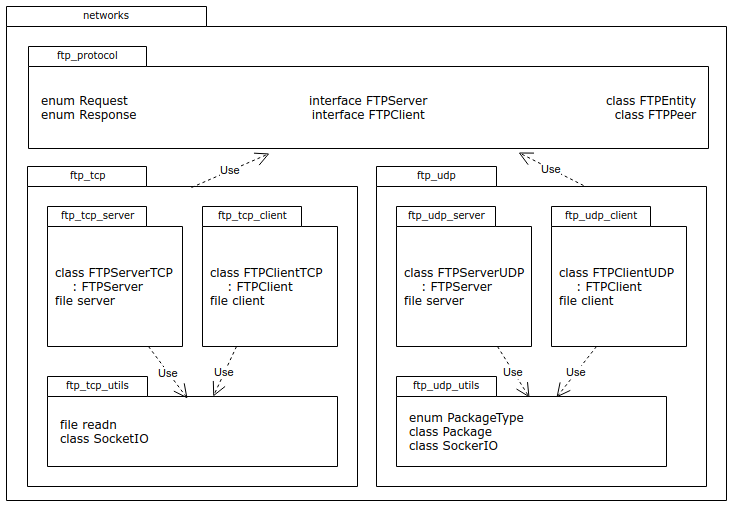
\includegraphics[width=\linewidth]{uml}
	\caption{Диаграмма модулей}
\end{figure}

Кроме того, независимо от реализации соединения был зафиксирован список поддерживаемых консольных команд серверного и клиентского приложений. Сервер поддерживает команды:
\begin{itemize}
	\item \code{list} -- отображение нумерованного списка подключенных клиентов;
	\item \code{kill <x>} -- принудительное отключение клиента с номером \code{x};
	\item \code{exit} -- завершения приема запроса от клиентов и завершение программы.
\end{itemize}

\noindent Клиентское приложение поддерживает консольные команды:
\begin{itemize}
	\item \code{connect <ip> <port>} -- подключение к серверному приложению, работающему по адресу \code{ip} и порту \code{port};
	\item \code{pwd} -- запрос имени текущей директории на сервере;
	\item \code{ls} -- запрос списка файлов в текущей директории на сервере;
	\item \code{cd <dir>} -- запрос на изменение текущей директории на сервере, формат совпадает с форматом команды \code{ls} в Linux;
	\item \code{get <file>} -- запрос на загрузку файла \code{file} с сервера;
	\item \code{put <file>} -- запрос на загрузку файла \code{file} на сервер;
	\item \code{disconnect} -- отключение от текущего сервера, что позволяет позже выполнить команду \code{connect} к другому серверу;
	\item \code{exit} -- завершение программы.
\end{itemize}

\subsection{Библиотечный модуль с описанием протокола}

В модуль \code{ftp\_protocol} содержит перечисления \code{Request} и \code{Response}, описывающий прикладной протокол, не зависящий от реализации:
\begin{itemize}
	\item \code{enum Request} -- перечисление, определяющее возможные типы запросов клиента серверу:
	\begin{itemize}
		\item \code{CONNECT} -- оповещение сервера о подключении (возможна реализация авторизации);
		\item \code{DISCONNECT} -- оповещение сервера о закрытии соединения;
		\item \code{PWD} -- запрос текущего пути на сервере;
		\item \code{LS} -- запрос списка файлов в текущей директории;
		\item \code{CD} -- запрос на изменение текущей директории на сервере;
		\item \code{GET} -- запрос на скачивание файла, имя которого указано в запросе;
		\item \code{PUT} -- запрос на загрузку файла, имя которого указано в запросе.
	\end{itemize}
	\item \code{enum Response} -- перечисление, определяющее возможные типы ответов сервера клиенту:
	\begin{itemize}
		\item \code{OK} -- успешно;
		\item \code{ERROR} -- ошибка общего типа;
		\item \code{NOT\_DIRECTORY} -- указывает на то, что путь, указанные при запросе \code{CD}, не указывал на директорию на сервере;
		\item \code{NOT\_REGULAR\_FILE} -- указывает на то, что запрошенный файл не является обычным файлом (например, директорией);
		\item \code{NOT\_EXISTS} -- указывает на то, что указанный в запросе файл не существует;
		\item \code{ALREADY\_EXISTS} -- указывает на то, что имя, указанное при загрузке файла на сервер, конфликтует с уже существующим файлом;
		\item \code{FILE\_DATA} -- указывает на то, что пакет содержит данные файла. Используется как клиентом, так и сервером;
		\item \code{FILE\_DATA\_END} -- указывает на то, что пакет является последним пакетом, содержащим данные файла. Используется как клиентом, так и сервером.
	\end{itemize}
\end{itemize}

\noindent Помимо перечислений модуль содержит вспомогательные классы для представления файла/директории и участника обмена соответственно:
\begin{itemize}
	\item \code{class FTPEntity} -- упрощает работу клиентскому приложению с получаемым списком сущностей (файлы и директории) и инкапсулирует в себе имя сущности и флаг, указывающий на то, является ли сущность директорией.
	\item \code{class FTPPeer} -- служит для идентификации участника обмена и инкапсулирует внутри себя IP-адрес и порт.
\end{itemize}

\noindent При помощи интерфейсов (чисто виртуальных классов в \code{C++}) \code{FTPServer} и \code{FTPClient} был зафиксирован список функций, которые должен поддерживать сервер и клиент независимо от реализации. Сервер должен определять функции:
\begin{itemize}
	\item \code{void connect()} -- обработка запроса на подключение;
	\item \code{void pwd()} -- обработка запроса на получение имени текущей директории;
	\item \code{void ls()} -- обработка запроса на получение списка файлов в текущей директории;
	\item \code{void cd()} -- обработка запроса на смену директории;
	\item \code{void get()} -- обработка запроса на загрузку файла с сервера;
	\item \code{void put()} -- обработка запроса на загрузку файла на сервер;
	\item \code{void disconnect()} -- обработка отключения клиента.
\end{itemize}

\noindent Клиент должен определять функции:
\begin{itemize}
	\item \code{connect(const std::string \&server\_addr, int port)} -- подключиться к серверу;
	\item \code{std::string pwd()} -- получить с сервера текущую директорию;
	\item \code{std::vector<FTPEntity> ls()} -- получить с сервера файлы в текущей директории;
	\item \code{void cd(const std::string \&string)} -- сменить директорию на сервере;
	\item \code{void get(const std::string \&file\_name)} -- загрузить файл с сервера;
	\item \code{void put(const std::string \&file\_name)} -- загрузить файл на сервер; 
	\item \code{disconnect()} -- отключиться от текущего сервера.
\end{itemize}

\subsection{Приложения на основе TCP}

Разработанный проект \code{ftp\_tcp} для удобства был разбит на модули:
\begin{itemize}
	\item \code{ftp\_tcp\_utils} -- библиотечный модуль, в который вынесена логика, общая для сервера и клиента;
	\item \code{ftp\_tcp\_server} -- серверной приложение, обеспечивающее функции обмена файлами;
	\item \code{ftp\_tcp\_client} -- приложение-клиент, обеспечивающее функции обмена файлами.
\end{itemize}

\subsubsection{Модуль \code{ftp\_tcp\_utils}}

В библиотечный модуль \code{utils} была вынесена логика, общая для модулей \code{ftp\_tcp\_server} и \code{ftp\_tcp\_client}:
\begin{itemize}
	\item \code{class SocketIO} -- класс, предоставляющий серверу и клиенту методы для отправки запросов и ответов поверх TCP и инкапсулирующий в себе работу с сокетом.
	\item \code{readn} -- функция, используемая в \code{SocketIO} для считывания нужного количества байт при чтении из сокета.

\end{itemize}

\subsubsection{Модуль \code{ftp\_tcp\_server}}

Модуль \code{ftp\_tcp\_server} представлет собой серверное приложение, обеспечивающее обработку запросов от нескольких клиентов:
\begin{itemize}
	\item \code{class FTPServerTCP : FTPServer} -- класс, предоставляющий обработчик запросов: в вечном цикле происходит принятие и обработка запросов клиента, а также формирование ответов.
	\item \code{server} -- файл, содержащий функцию \code{main} и основную логику принятия соединений, создания экземпляров \code{FTPServerTCP} и получения команд из консоли.
\end{itemize}

\subsubsection{Модуль \code{ftp\_tcp\_client}}

Модуль \code{ftp\_tcp\_client} представляет собой клиентское приложение, позволяющее формировать запросы и получать ответы от серверного приложения:
\begin{itemize}
	\item \code{class FTPClientTCP : FTPClient} -- класс, формирующий запросы к серверу и интерпретирующий ответы сервера.
	\item \code{client} -- файл, содержащий функцию \code{main} и основную логику обработки пользовательских команд, введенных в консоль.
\end{itemize}

\subsection{Приложения на основе UDP}

Приложение, построенное на основе UDP \code{ftp\_udp} аналогичным образом было разбито на модули:
\begin{itemize}
	\item \code{ftp\_udp\_utils} -- библиотечный модуль, в который вынесена логика, общая для сервера и клиента;
	\item \code{ftp\_udp\_server} -- серверной приложение, обеспечивающее функции обмена файлами;
	\item \code{ftp\_udp\_client} -- приложение-клиент, обеспечивающее функции обмена файлами.
\end{itemize}

\subsubsection{Модуль \code{ftp\_udp\_utils}}

Из-за особенностей UDP протокола возникла потребность в еще одном уровне вложенности пересылаемых пакетов. Был добавлен класс \code{Package}, включающий в себя номер пакета (необходим для отслеживания доставки и отправки подтверждения), тип пакета (запрос ответ, подтверждение или пустой пакет), код запроса или ответа и массив данных. В TCP такая потребность отсутствовала, потому что пересылаемые данные не делились на пакеты, а передавались потоков байт.

\begin{itemize}
	\item \code{enum PackageType} -- перечисление, определяющее возможные типы пакетов при общении клиента и сервера:
	\begin{itemize}
		\item \code{REQUEST} -- запрос;
		\item \code{RESPONSE} -- ответ;
		\item \code{ACK} -- подтверждение о получении пакета;
		\item \code{EMPTY} -- пустой пакет, служит для идентификации того, что пакет получить не удалось или возникла ошибка в процессе разбора пакета.
	\end{itemize}
	\item \code{class Package} -- является единицой пересылки между клиентом и сервером. Класс включает в себя:
	\begin{itemize}
		\item счетчик \code{size\_t counter}, являющийся уникальным числом для всех пакетов;
		\item тип пакета \code{PackageType packageType};
		\item код запроса (\code{Request}) или ответа (\code{Response}) \code{reqresp};
		\item указатель на массив байт \code{char* data}, представляющие собой передаваемые данные.
	\end{itemize}
	\item \code{class SocketIO} -- класс, предоставляющий серверу и клиенту методы для отправки запросов и ответов поверх UDP и инкапсулирующий в себе работу с сокетом.
\end{itemize}

\subsubsection{Модуль \code{ftp\_udp\_server}}

Модуль \code{ftp\_udp\_server} представлет собой серверное приложение, обеспечивающее обработку запросов от нескольких клиентов:
\begin{itemize}
	\item \code{class FTPServerUDP : FTPServer} -- класс, предоставляющий обработчик запросов: по мере поступления запросов от клиента происходит их обработка, а также формирование ответов.
	\item \code{server} -- файл, содержащий функцию \code{main} и основную логику принятия соединений, создания экземпляров \code{FTPServerTCP} и получения команд из консоли.
\end{itemize}

\subsubsection{Модуль \code{ftp\_tcp\_client}}

Модуль \code{ftp\_udp\_client} представляет собой клиентское приложение, позволяющее формировать запросы и получать ответы от серверного приложения:
\begin{itemize}
	\item \code{class FTPClientUDP : FTPClient} -- класс, формирующий запросы к серверу и интерпретирующий ответы сервера.
	\item \code{client} -- файл, содержащий функцию \code{main} и основную логику обработки пользовательских команд, введенных в консоль.
\end{itemize}

\section{Особенности реализации}

% Особенности реализации сетевых и многопоточных приложений: readn, завершение потоков, мьютексы и др.

\subsection{Приложения на основе TCP}

\subsubsection{Серверное приложение}

При запуске серверного приложения в главном потоке создается серверный TCP сокет, привязывается к 7000 порту и переводится в режим прослушивания. После этого создается поток \code{acceptThread} занимающийся приемом соединений через серверный сокет. Затем главный поток начинает в вечном цикле принимать команды с консоли для управления текущими подключениями. По окончанию ввода команд (получении команды exit), главный поток дожидается окончания потока \code{acceptThread}.

Поток приема соединений \code{acceptThread} в вечном цикле принимает подключения через серверный сокет и для каждого нового клиента создает экземпляр класса \code{FTPServerTCP} и клиентский поток \code{clientThread}. Экземляр созданного класса добавляется в глобальный список активных серверов. Затем происходит запуск клиентского потока. 

Поток \code{clientThread} вызывает функцию \code{processRequest} экземпляра класса \code{FTPServerTCP}, получаемого через аргументы, и производит обработку возникающих исключений. По окончании общения клиента и сервера клиентский поток удаляет себя из списка активных серверов и завершается.

Синхронизация доступа к глобальному списку активных серверов из разных потоков достигается при помощи использования \code{pthread\_rwlock} -- блокировки по чтению-записи. Данный примитив позволяет блокировать доступ к общей переменной на запись или на чтение, при этом читать могут сразу несколько потоков.

\subsubsection{Клиентское приложение}

Клиентское приложение является однопоточным. При старте клиентского приложения создается экземпляр класса \code{FTPClientTCP}, к которому направляются соответствующие запросы с консоли. Экземпляр класса инкапсулирует в себе формирование соответствующих запросов серверу. 

И клиентское, и серверное приложение используют класс \code{SocketIO} для отправки и получения запросов и ответов. Класс \code{SocketIO} использует для отправки данных системный вызов \code{send()}, а для получения -- функцию \code{readn()}, которая является надстройкой над системным вызовом \code{recv()}. Это необходимо для того, чтобы принимать именно то количество байт, которое необходимо согласно протоколу.


\subsection{Приложения на основе UDP}

\subsubsection{Серверное приложение}

При запуске серверного приложения в главном потоке создается UDP сокет и привязывается к 7000 порту. После этого создается и запускается поток для обработки запросов \code{processingThread}. Главный поток заходит в вечный цикл и начинает считывать управляющие команды с консоли. После получения команды exit, из списка активных серверов удаляются все обработчики, происходит ожидание завершения потока \code{processingThread} и приложение завершается.

Поток \code{processingThread} в вечном цикле получает пакеты, используя класс \code{SocketIO}, инкапсулирующий в себе получение, отправку и разбор UDP-пакетов. При получении пакета (экземпляра класса \code{Package}) происходит поиск существующего экземпляра \code{FTPServerUDP} для отправителя (отправитель представлен экземпляром \code{FTPPeer}) и если сервер отсутствует, он создается и сохраняется в отображении \code{std::map<FTPPerr, FTPServerUDP *>}. Полученный пакет передается серверу для обработки запроса. Таким образом, реализована однопоточная обработка запросов, что является узким местом в данной реализации.

\subsubsection{Клиентское приложение}

Клиентское приложение для UDP ничем не отличается от TCP, за исключением типа создаваемого клиентского обработчика запросов -- вместо \code{FTPClientTCP} создается экземпляр класса \code{FTPClientUDP}, к котором инкапсулируется создание пакетов для отправки серверу.

И клиентское, и серверное приложение используют класс \code{SocketIO} для отправки и получения запросов и ответов. Класс \code{SocketIO} использует для отправки данных системный вызов \code{sendto()}, а для получения -- функцию \code{recvfrom()}. Кроме того, \code{SocketIO} обеспечивает вызывающей стороне отправку подтверждений на приходящие пакеты и гарантию доставки отправляемых пакетов другой стороне. Это достигается за счет блокирования потока выполнения на определенный интервал времени (при помощи вызова функции \code{select()} с заданным таймаутом) после отправки пакета до получения пакета с подтверждением. Если в течении одной секунды не приходит подтверждение на отправленный пакет, \code{SocketIO} отправляет его еще раз, после чего блокируется на секунду снова.

\section{Результаты тестирования}

% Результаты тестирования приложения (с разным набором входных данных, методика тестирования параллельности обработки запросов клиентов, проверка программы на потерю, дублирование и перемешивание дейтаграмм).

\subsection{Приложение на основе TCP}

Для тестирования разработанного приложения на основе TCP были запущены серверное и 3 клиентских приложения. Клиенты одновременно отправляли запросы на получение большого файла (6 ГБ). Сервер успешно параллельно обрабатывал запросы всех клиентов и параллельно отправлял файлы разным клиентам. 

После этого были протестированы функции принудительного отключения выбранного клиента. После выполнения команды \code{kill} клиентский сокет на сервере зарывался, а клиентский поток успешно завершался. Клиенту при этом выводилось сообщение о его принудительном отключении от сервера.

Было протестировано завершение серверного приложения, клиентские сокеты и клиентские потоки успешно завершались, при этом происходило ожидание завершения потоков.

Приведем краткий пример взаимодействия клиента с сервером:
\lstinputlisting{logs/tcpcli.txt}

\lstinputlisting{logs/tcpser.txt}

\subsection{Приложение на основе UDP}

Для тестирования приложений на основе UDP были выполнены аналогичные действия (подключение нескольких клиентов, принудительное отключение клиента и корректное завершение сервера). Кроме того, были рассмотренны особые тестовые сценарии:
\begin{itemize}
	\item Для проверки сервера

	\begin{itemize}
		\item Отправка дейтаграмм в неправильном порядке
		
		Для этого на клиенте было добавлено условие: при отправке запроса \code{pwd} к номеру пакета был добавлено 100, имитируя ошибку в порядке прихода дейтаграмм. Видно, что сервер отбросил дейтаграмму с неверным номером.
		
		\lstinputlisting[language=none]{logs/udpordcli.txt}
		\lstinputlisting[language=none]{logs/udpordsrv.txt}
		
		\item Отправка дейтаграмм-дубликатов
		
		Для этого на клиенте было добавлено условие: при отправке запроса \code{pwd} пакет с запросом отправлялся дважды. Видно, что за счет нумерации пакетов, сервер отбросил пакет-дубликат.
		
		\lstinputlisting[language=none]{logs/udpdupcli.txt}
		\lstinputlisting[language=none]{logs/udpdupsrv.txt}
		
		\item Пропуск дейтаграмм для имитации потерь
		
		Для этого клиент однократно не отправляем пакет с \code{ACK} на пришедший пакет с номером 7. Видно, что сервер корректно обработал эту ситуацию и повторно отправил 7-ой пакет, на которой уже был получен \code{ACK}.
		
		\lstinputlisting[language=none]{logs/udpmiscli.txt}
		\lstinputlisting[language=none]{logs/udpmissrv.txt}
	\end{itemize}
	Таким образом серверное приложение корректно справилось с заготовленными сценариями.
	
	\item Для проверки клиента на сервере было добавлено условие, при котором если номер пакета равен 4, то \code{ACK} для него не отсылался. Клиент пытался 5 раз с интервалом в 1 секунду отправить запрос, после чего попытки отправить запрос прекращались и пользователю выводилось сообщение об ошибке.
	
	\lstinputlisting[language=none]{logs/udpackcli.txt}
	\lstinputlisting[language=none]{logs/udpacksrv.txt}

\end{itemize}

\section{Выводы}

% Раздел «Выводы» должен включать в себя содержательные выводы, сделанные именно по данной работе. Здесь следует подчеркнуть особенности используемых протоколов, режимов работы, применяемых технологий и библиотек.

В процессе выполнения работы был придуман прикладной протокол для системы передачи файлов: были определены форматы запроса и ответа. По описанию протокола были составлены интерфейсы клиентского и серверного приложений.

Было реализовано два клиент-серверных приложения, поддерживающих обмен данными по прикладному протоколу, поверх протокола TCP и UDP. За счет инкапсуляции логики обмена данными внутри класса \code{SocketIO}, некоторые части приложений одинаковы для TCP и UDP. Различным оказалась работа на уровне сокетов. За счет необходимости отслеживания доставки пакетов, реализация прикладного протокола на UDP оказалось более сложной.

Исходный код разработанных приложений размещен в Git репозитории: 
\url{https://github.com/vaddya/computer-networks}

\newpage

\section*{Приложение. Исходный код приложений}

\lstinputlisting[caption=\code{ftp\_server.h}]{../ftp_protocol/ftp_server.h}

\lstinputlisting[caption=\code{ftp\_client.h}]{../ftp_protocol/ftp_client.h}

\lstinputlisting[caption=\code{request.h}]{../ftp_protocol/request.h}

\lstinputlisting[caption=\code{request.h}]{../ftp_protocol/response.h}

\lstinputlisting[caption=\code{ftp\_entity.h}]{../ftp_protocol/ftp_entity.h}

\lstinputlisting[caption=\code{ftp\_peer.h}]{../ftp_protocol/ftp_peer.h}


\lstinputlisting[caption=\code{ftp\_server\_tcp.h}]{../ftp_tcp/server/ftp_server_tcp.h}

\lstinputlisting[caption=\code{ftp\_server\_tcp.cpp}]{../ftp_tcp/server/ftp_server_tcp.cpp}

\lstinputlisting[caption=\code{ftp\_tcp/server.h}]{../ftp_tcp/server/server.h}

\lstinputlisting[caption=\code{ftp\_tcp/server.cpp}]{../ftp_tcp/server/server.cpp}


\lstinputlisting[caption=\code{ftp\_client\_tcp.h}]{../ftp_tcp/client/ftp_client_tcp.h}

\lstinputlisting[caption=\code{ftp\_client\_tcp.cpp}]{../ftp_tcp/client/ftp_client_tcp.cpp}

\lstinputlisting[caption=\code{ftp\_tcp/client.h}]{../ftp_tcp/client/client.h}

\lstinputlisting[caption=\code{ftp\_tcp/client.cpp}]{../ftp_tcp/client/client.cpp}



\lstinputlisting[caption=\code{ftp\_server\_udp.h}]{../ftp_udp/server/ftp_server_udp.h}

\lstinputlisting[caption=\code{ftp\_server\_udp.cpp}]{../ftp_udp/server/ftp_server_udp.cpp}

\lstinputlisting[caption=\code{ftp\_udp/server.h}]{../ftp_udp/server/server.h}

\lstinputlisting[caption=\code{ftp\_udp/server.cpp}]{../ftp_udp/server/server.cpp}


\lstinputlisting[caption=\code{ftp\_client\_udp.h}]{../ftp_udp/client/ftp_client_udp.h}

\lstinputlisting[caption=\code{ftp\_client\_udp.cpp}]{../ftp_udp/client/ftp_client_udp.cpp}

\lstinputlisting[caption=\code{ftp\_udp/client.h}]{../ftp_udp/client/client.h}

\lstinputlisting[caption=\code{ftp\_udp/client.cpp}]{../ftp_udp/client/client.cpp}

\end{document}
